\documentclass[a4paper,12pt]{article}
\usepackage[a4paper, margin=1in]{geometry} % Sets the paper size to A4 and margins to 1 inch
\usepackage{graphicx}
\usepackage{subcaption} % for subfigures
\usepackage{setspace}		
\usepackage{xcolor,listings} % for typesetting code
\usepackage{enumitem}
\usepackage{tabularx}

% Define SQL listing style
% \lstset{
%     language=SQL,
%     basicstyle=\ttfamily,
%     keywordstyle=\bfseries,
%     commentstyle=\itshape,
%     showstringspaces=false,
%     numbers=left,
%     numberstyle=\tiny,
%     numbersep=5pt,
%     breaklines=true,
%     frame=single,
%     backgroundcolor=\color{gray!10},
%     captionpos=b
% }
\lstset{
    upquote=true,
    language=SQL,
    showspaces=false,
    basicstyle=\ttfamily,
    keywordstyle=\bfseries\color{blue!50},
    numbers=left,
    numberstyle=\tiny,
    commentstyle=\color{gray},
    backgroundcolor=\color{gray!10}
}

\begin{document}


%% Adding logo
\begin{figure}[h]
		\vspace*{-1em}
		\centering
		
\includegraphics[width=0.2\linewidth]{university_logo.png}
		\par
		\vspace*{2em}
		{\Large UNIVERSITY OF CHITTAGONG}
\end{figure}
%% Document information
\begin{center}
		\vspace*{3em}
		\textbf{Department of Computer Science and Engineering} \\
		\bigskip
		Session: 2021-2022 \\
		4th semester \\
		\bigskip
		\begin{tabular}{l l}
		  Assignment No. &: 1\\
		  Course Title &: Database Systems \\
		  Course Code No. &: CSE-413 \\
		\end{tabular}
\end{center}

%% Teacher information
\begin{center}
		\vspace*{3em}
		Submitted to: \\
		\textbf{Dr. Rudra Pratap Deb Nath} \\
		Associate Professor \\
		Department of Computer Science and Engineering \\
		University of Chittagong
\end{center}

%% Student information
\begin{center}
		\vspace*{3em}
		Submitted by: \\
		\textbf{Sanzid Islam Mahi} \\
		ID: 22701065 \\
		Department of Computer Science and Engineering \\
		University of Chittagong
\end{center}




\begin{center}
	\vspace*{3em}
	Date: Jul 02, 2024
\end{center}

\newpage
\section*{Chapter 3}
\subsection*{Practice 3}
\begin{enumerate}
    \item Create a report that produces the following for each employee: \\
\textless employee last name\textgreater{} earns \textless salary\textgreater{} monthly but wants \textless 3 times
salary.\textgreater{}. Label the column Dream Salaries.

    \begin{figure}[h]
        \centering
            \centering
            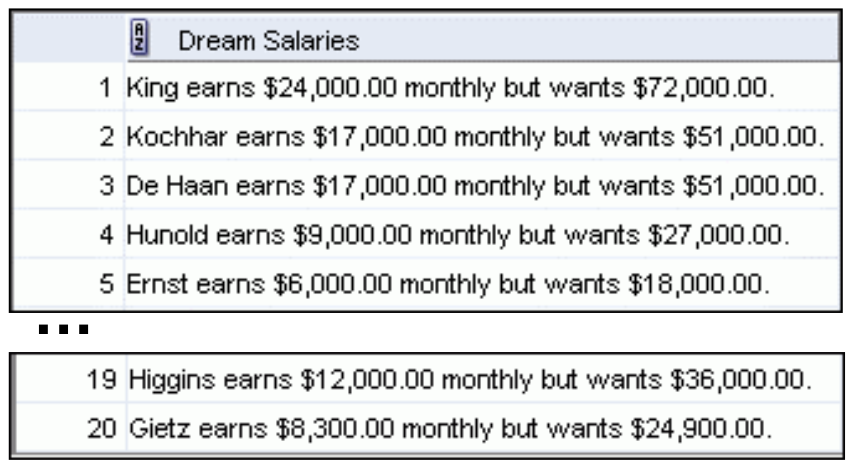
\includegraphics[width=.5\linewidth]{graphics/41.png}
    \end{figure}
    
    \textbf{Solution: }
    \begin{lstlisting}[language=SQL]
SELECT Last_Name || ' earns ' || Salary || 
    ' monthly but wants ' || (Salary * 3) || '.' 
    AS "Dream Salaries"
FROM hr.Employees;
    \end{lstlisting}
        \item Display each employee's last name, hire date, and salary review date, which is the first Monday
after six months of service. Label the column REVIEW. Format the dates to appear in the format
similar to “Monday, the Thirty-First of July, 2000.”

    \begin{figure}[h]
        \centering
            \centering
            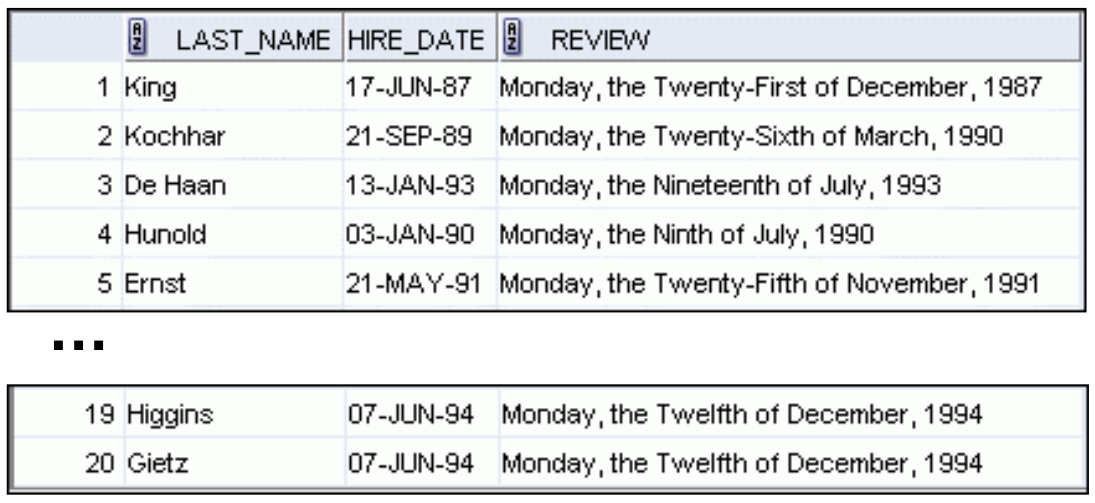
\includegraphics[width=.6\linewidth]{graphics/42.png}
    \end{figure}
    
    \textbf{Solution: }
    \begin{lstlisting}[language=SQL]
SELECT 
    last_name,
    hire_date,
    TO_CHAR(
        NEXT_DAY(ADD_MONTHS(hire_date, 6) - 1, 'MONDAY'),
        'FMDay,"the" fmDdsp "of" FMMonth,YYYY'
    ) AS review
FROM 
    hr.employees;
    \end{lstlisting}
    \item Display the last name, hire date, and day of the week on which the employee started. Label the
column DAY. Order the results by the day of the week, starting with Monday.
    \begin{figure}[h]
        \centering
            \centering
            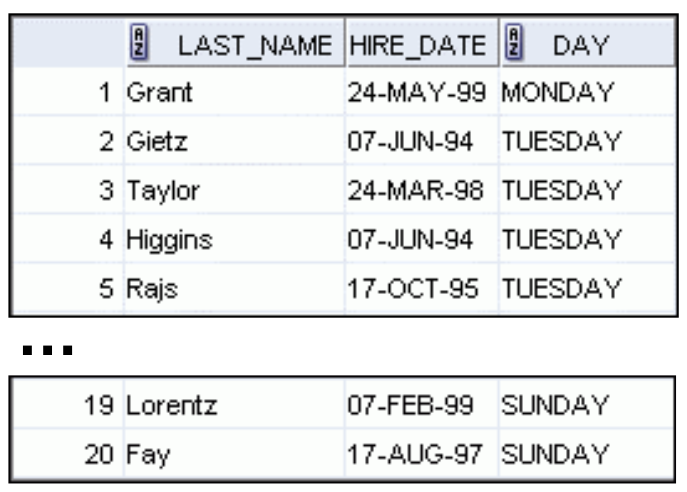
\includegraphics[width=.5\linewidth]{graphics/43.png}
    \end{figure}
    
    \textbf{Solution: }
    \begin{lstlisting}[language=SQL]
SELECT Last_Name || ' earns ' || Salary || 
    ' monthly but wants ' || (Salary * 3) || '.' 
    AS "Dream Salaries"
FROM hr.Employees;
    \end{lstlisting}
        \item Create a query that displays the employees' last names and commission amounts. If an employee
does not earn commission, show “No Commission.” Label the column COMM.
    \begin{figure}[h]
        \centering
            \centering
            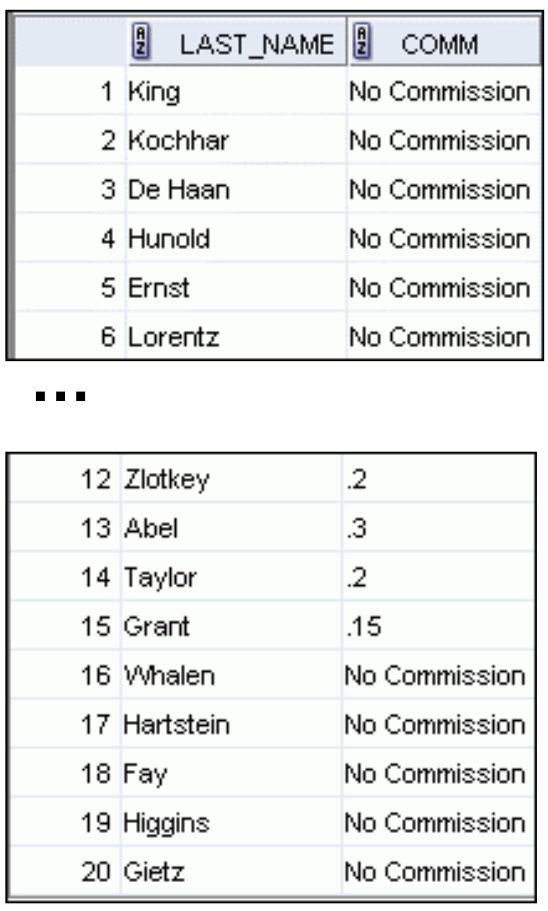
\includegraphics[width=.4\linewidth]{graphics/44.png}
    \end{figure}
    
    \textbf{Solution: }
    \begin{lstlisting}[language=SQL]
SELECT last_name,
    CASE 
        WHEN commission_pct IS NULL OR commission_pct = 0 
        THEN 'No Commission'
        ELSE TO_CHAR(commission_pct,'fm.99')
    END AS comm
FROM 
    hr.employees;
    \end{lstlisting}
        \item Using the DECODE function, write a query that displays the grade of all employees based on the
value of the column \texttt{JOB\_ID}, using the following data:
 
\begin{tabularx}{\textwidth}{lX}
\textbf{Job} & \textbf{Grade} \\
AD\_PRES & A \\
ST\_MAN & B \\
IT\_PROG & C \\
SA\_REP & D \\
ST\_CLERK & E \\
None of the above & 0 \\
\end{tabularx}
    
    \begin{figure}[h]
        \centering
            \centering
            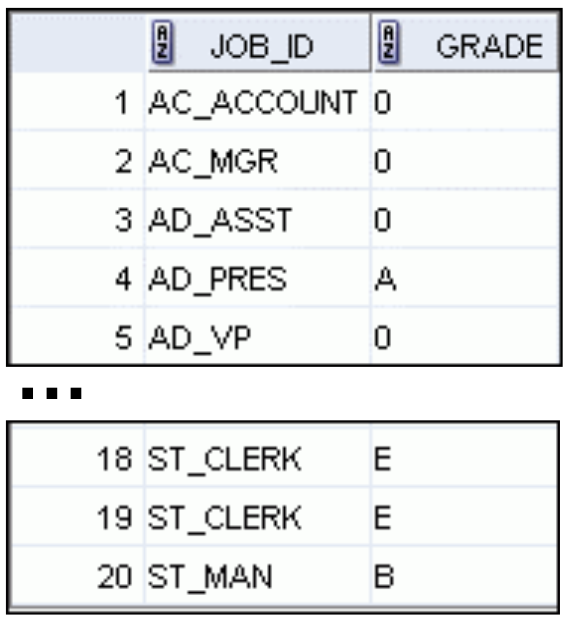
\includegraphics[width=.3\linewidth]{graphics/45.png}
    \end{figure}

    \textbf{Solution: }
    \begin{lstlisting}[language=SQL]
SELECT last_name,job_id,
    DECODE(job_id,
           'AD_PRES', 'A',
           'ST_MAN', 'B',
           'IT_PROG', 'C',
           'SA_REP', 'D',
           'ST_CLERK', 'E',
           '0'
    ) AS grade
FROM hr.employees;
    \end{lstlisting}
    \item Rewrite the statement in the preceding exercise using the CASE syntax.
    \begin{figure}[h]
        \centering
            \centering
            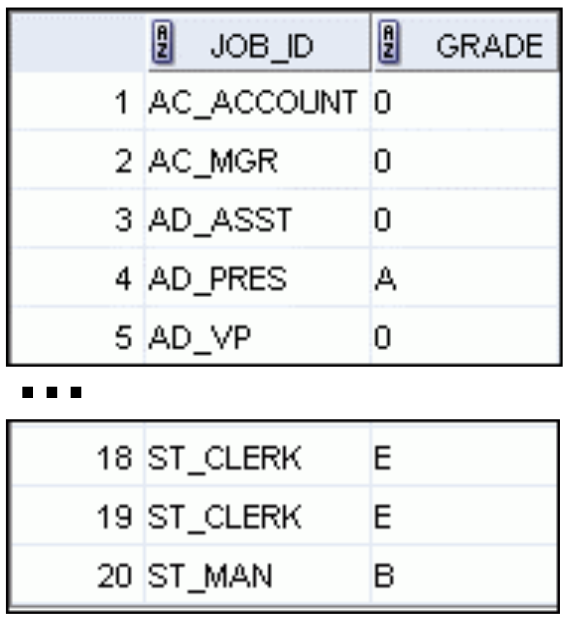
\includegraphics[width=.3\linewidth]{graphics/46.png}
    \end{figure}
    
    \textbf{Solution: }
    \begin{lstlisting}[language=SQL]
SELECT last_name,job_id,
    CASE job_id
        WHEN 'AD_PRES' THEN 'A'
        WHEN 'ST_MAN' THEN 'B'
        WHEN 'IT_PROG' THEN 'C'
        WHEN 'SA_REP' THEN 'D'
        WHEN 'ST_CLERK' THEN 'E'
        ELSE '0'  -- Default case for other values
    END AS grade
FROM employees;

    \end{lstlisting}
\end{enumerate}
\end{document}
